% path to figures directory
\graphicspath{{img/chapter_1/}}

\chapter{Introduction}
\label{chapter:introduction}

\begin{flushleft}
  \textit{The following is a general introduction to the background topics
    referred to and assumed in subsequent chapters. This includes a review of
    popular theories of neutrino mass, the current status of
    neutrino-oscillation parameters, a general introduction to Effective Field
    Theory (EFT), the experimental situation relevant to the flavour anomalies,
    and topics peripheral to all of these.}
\end{flushleft}

\section{The Standard Model and neutrinos}

Laboratory experiments to date have firmly established the predictive power of
the Standard Model (SM) of particle physics, a combined theory of the
electroweak and strong interactions described by the gauge group
$G_{\text{SM}} = \mathrm{SU}(3)_{c} \otimes \mathrm{SU}(2)_{L} \otimes \mathrm{U}(1)_{Y}$.
It is a model whose probes and predictions span at least 33 orders of
magnitude\footnote{The interval given is from the distance scales probed at the
  LHC (roughly $\SI{e-17}{\cm}$) to the size of the solar system (roughly
  \SI{e16}{\cm}).} with varying degrees of precision, and these are consistent
with almost all known experiments. Although it displays a number of arbitrary
features, the dynamics of the theory are mostly fixed by the fundamental
principles of gauge theory and Lorentz invariance. Most of this arbitrariness
resides in the matter sector of the theory, whose properties (masses, coupling
constants, quantum numbers, \textit{etc.}) are not predicted, but are instead
motivated on phenomenological grounds. We show the fields of the SM and their
defining properties in Table~\ref{tab:sm-fields}, according to the mathematical
conventions of Appendix~\ref{chapter:notation}.
\begin{table}[t]
  \centering
  \bgroup
  \def\arraystretch{1.3}% 1 is the default
  \begin{tabular}{ccc}
    \toprule
    Field                        & $\mathrm{SU}(3)_{c} \otimes \mathrm{SU}(2)_{L} \otimes \mathrm{U}(1)_{Y}$ & $\mathrm{SU}(2)_{+} \otimes \mathrm{SU}(2)_{-}$ \\
    \midrule
    $Q^{\alpha a i}$             & $(\mathbf{3}, \mathbf{2}, \tfrac{1}{6})$                                  & $(\mathbf{2}, \mathbf{1})$                      \\
    $L^{\alpha i}$               & $(\mathbf{1}, \mathbf{2}, -\tfrac{1}{2})$                                 & $(\mathbf{2}, \mathbf{1})$                      \\
    $\bar{u}^{\alpha}_a$                  & $(\bar{\mathbf{3}}, \mathbf{1}, -\tfrac{2}{3})$                           & $(\mathbf{2}, \mathbf{1})$                      \\
    $\bar{d}^{\alpha}_a$                  & $(\bar{\mathbf{3}}, \mathbf{1}, \tfrac{1}{3})$                            & $(\mathbf{2}, \mathbf{1})$                      \\
    $\bar{e}^{\alpha}$                    & $(\mathbf{1}, \mathbf{1}, 1)$                                             & $(\mathbf{2}, \mathbf{1})$                      \\
    $(G_{\alpha \beta})^a_{\ b}$ & $(\mathbf{8}, \mathbf{1}, 0)$                                             & $(\mathbf{3}, \mathbf{1})$                      \\
    $(W_{\alpha \beta})^i_{\ j}$ & $(\mathbf{1}, \mathbf{3}, 0)$                                             & $(\mathbf{3}, \mathbf{1})$                      \\
    $B_{\alpha \beta}$           & $(\mathbf{1}, \mathbf{1}, 0)$                                             & $(\mathbf{3}, \mathbf{1})$                      \\
    $H^{i}$                      & $(\mathbf{1}, \mathbf{2}, \tfrac{1}{2})$                                  & $(\mathbf{1}, \mathbf{1})$                      \\
    \bottomrule
  \end{tabular}
  \egroup
  \caption{The SM fields and their transformation properties under the SM gauge
    group $G_{\text{SM}}$ and the Lorentz group written as
    $\mathrm{SU}(2)_{+} \otimes \mathrm{SU}(2)_{-}$. The final unbolded number
    in the 3-tuples of the $G_{\text{SM}}$ column represents the
    $\mathrm{U}(1)_Y$ charge of the field, normalised such that $Q = I_{3} + Y$.
    For the fermions a generational index has been suppressed. See
    Appendix~\ref{chapter:notation} for details about the mathematical notation
    used here and throughout this work.}
  \label{tab:sm-fields}
\end{table}

The SM inherits the experimental success of the
$\mathrm{SU}(2) \otimes \mathrm{U}(1)$ theory of the weak interactions, first
proposed by Glashow~\cite{Glashow:1961tr} in 1961 as a possible underlying
structure for Fermi's theory of beta decay. Before the end of the same decade,
Weinberg~\cite{Weinberg:1967tq} and Salam~\cite{Salam:1968rm} had constructed
the modern theory of leptons based on the spontaneous breaking of
$\mathrm{SU}(2)_{L} \otimes \mathrm{U}(1)_{Y}$ to the electromagnetic symmetry.
Interestingly, it seems that these seminal papers went mostly unnoticed (see
Fig.~\ref{fig:weinberg-citations}) until the early 1970s, when 't~Hooft proved
the renormalisability of spontaneously broken gauge
theories~\cite{tHooft:1971akt} as a graduate student working under the
supervision of Veltman. By the mid 1970s the framework had been extended to
include the quarks~\cite{Glashow:1970gm} and the unbroken chromodynamic group,
which was successfully shown to reproduce the Bjorken scaling seen in
deep-inelastic-scattering experiments through asymptotic
freedom~\cite{Gross:1973id}.
\begin{figure}[t]
  \centering
  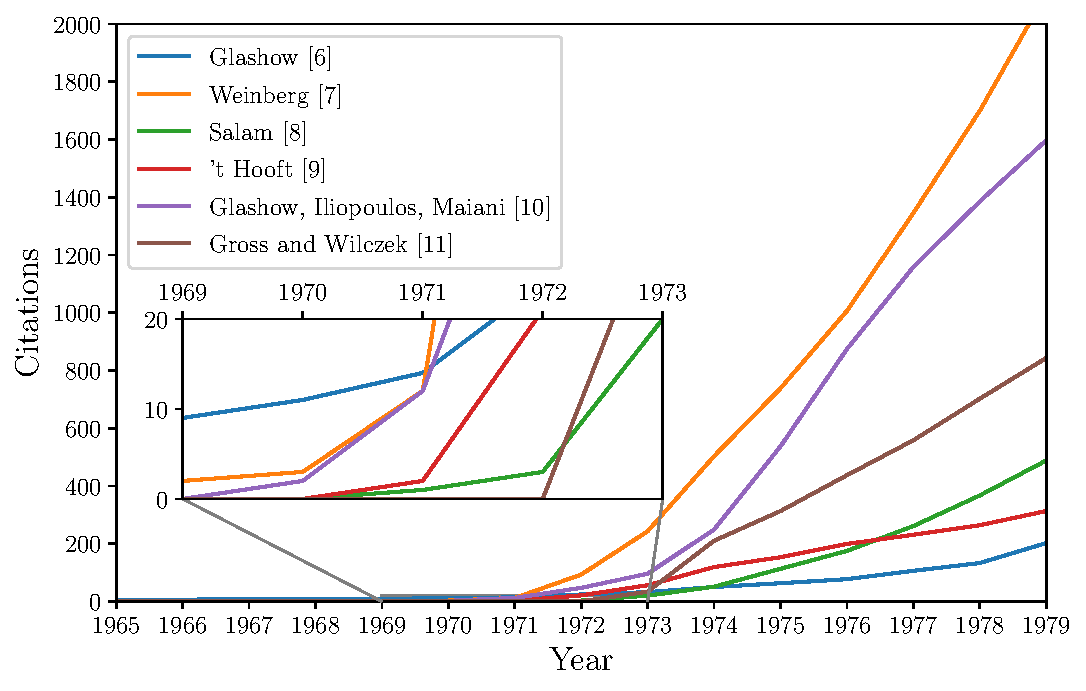
\includegraphics[width=0.9\linewidth]{weinberg_citations}
  \caption{The cumulative citation graph for a selection of papers presenting
    foundational results relevant to the SM. Weinberg's seminal paper `A model
    of leptons' (1967) saw an explosion of citations following 't~Hooft's work
    on the renormalisability of gauge theories (1971).}
  \label{fig:weinberg-citations}
\end{figure}

Despite its successes, the SM cannot be the complete theory of fundamental
particles and their interactions. It does not explain phenomena such as the
baryon asymmetry present in the Universe or its accelerating expansion.
Additionally, the particle spectrum contains no viable candidate for dark
matter, whose existence is strongly suggested by astrophysical and cosmological
data. The SM cannot explain why the electric dipole moment of the neutron is so
small, why there are three generations of matter or, notably in our case, the
origin of neutrino oscillations and the implied small but non-zero neutrino
masses.

\section{Massive neutrinos in experiment and theory}

In the SM the neutrino fields appear only within the lepton doublet $L$, and one
cannot write down---in analogy to the up-type Yukawa---a renormalisable operator
that leads to neutrino masses because of the absence of the right-handed fields.
The wealth of experimental evidence for massive neutrinos then constitutes clear
evidence for physics beyond the SM.

This evidence could in principle have come from many kinds of experiments, but
currently only neutrino oscillations provide strong signs that the masses are
non-zero. Below we discuss the phenomenon of neutrino oscillations in the
context of the outstandingly successful three-flavour mixing paradigm. We then
move on to other probes of neutrino masses, which currently only provide limits
on the mass scale. On the theory side, we summarise some popular and motivated
extensions of the SM that accommodate massive neutrinos, placing particular
emphasis on the direction we have followed in the novel work presented in this
thesis. This includes an overview of tree- and loop-level models of Majorana
neutrino mass.

\subsection{Neutrino oscillations}

The neutrino flavour eigenstates $\breve{\nu}_{i}$ =
$(\nu_{e}, \nu_{\mu}, \nu_{\tau})$ are defined as the states that couple at
charged-current interaction vertices with the corresponding charged lepton.
These are the states in which the neutrinos are almost always produced in
experiments, and certainly always measured. If neutrinos are massive there is no
reason to expect these to coincide with the mass eigenstates
$\nu_{i} = (\nu_{1}, \nu_{2}, \nu_{3})$. In general, the flavour eigenstates
will be an admixture of the propagating fields
\begin{equation}
  \label{eq:neutrino-mixing}
  \breve{\nu}_{i} = U_{i}^{* j} \nu_{j} \ ,
\end{equation}
where the $U_{i}^{\ j}$ are elements of the unitary
Pontecorvo--Maki--Nakagawa--Sakata (PMNS) neutrino mixing
matrix~\cite{Pontecorvo:1957cp, Maki:1962mu}. The PMNS matrix is defined such
that it diagonalises the neutrino mass matrix:
\begin{equation}
  \mathbf{U}^{\dagger} \mathbf{m}_{\nu} \mathbf{U}^{*} = \mathrm{diag}(m_{1}, m_{2}, m_{3}),
\end{equation}
where the $m_i$ are the neutrino masses. Being a $3 \times 3$ unitary matrix,
$\mathbf{U}$ is in general parametrised by three mixing angles and six phases.
Not all of the phases are physical, since the neutrino and charged-lepton fields
can be redefined in such a way that five of the phases are removed in the case
of Dirac neutrinos. In the presence of a Majorana mass term, only the charged
leptons can be rephased. This leaves three physical phases with the two
additional ones termed \textit{Majorana phases}. In general
\begin{equation}
  \label{eq:pmns}
  \mathbf{U} =
  \begin{bmatrix}
    c_{12}c_{13} & s_{12} c_{13} & s_{13}e^{-i\delta_\text{CP}} \\
    -s_{12}c_{23} - c_{12}s_{23}s_{13}e^{i\delta_\text{CP}} & c_{12}c_{23} - s_{12}s_{23}s_{13}e^{i\delta_\text{CP}} & s_{23}c_{13}\\
    s_{12}s_{23} - c_{12}c_{23}s_{13}e^{i\delta_\text{CP}} & -c_{12}s_{23} - s_{12}c_{23}s_{13}e^{i\delta_\text{CP}} & c_{23}c_{13}
  \end{bmatrix}
  \mathbf{P} \ ,
\end{equation}
where $c_{ij} = \cos \theta_{ij}$, $s_{ij} = \sin \theta_{ij}$ and
\begin{equation}
  \mathbf{P} =
  \begin{cases}
    \mathrm{diag}(e^{i \alpha_{1}}, e^{i \alpha_{2}}, 1) & \text{for Majorana neutrinos} \\
    \mathbf{1}_{3 \times 3} & \text{for Dirac neutrinos} \\
  \end{cases} \ .
\end{equation}
The phase $\delta_{\text{CP}}$ is often called the \textit{Dirac phase}, while
$\alpha_{1,2}$ are the Majorana phases discussed above.

Neutrino oscillation experiments typically involve the production of neutrino
flavour states from charged-current processes, \textit{e.g.} leptonic pion
decays. Each mass eigenstate evolves in time independently according to the
Schr\"{o}dinger equation: \textit{i.e.}
$| \nu_{i} (t) \rangle = \exp{(-i E_{i} t)} | \nu_{i} (0) \rangle$, for evolution
\textit{in vacuo}. This alters the initial superposition away from being a pure
flavour eigenstate:
\begin{align}
  | \breve{\nu}_{i} (t) \rangle &= \sum_{j} U_{i}^{* j} e^{-i E_{j} t} | \nu_{j} \rangle \\
                                &= \sum_{j,k} U_{i}^{* j} e^{-i E_{j} t} U_{j}^{\ k} | \breve{\nu}_{k} \rangle \ .
\end{align}
The probability of measuring a specific flavour through the charged-current
interaction then oscillates with time:
\begin{equation}
  \text{P}(\breve{\nu}_{m} \to \breve{\nu}_{n}) = | \langle \breve{\nu}_{n} | \breve{\nu}_{m} (t) \rangle |^{2} = \left| \sum_{i} U_{m}^{* i} U_{i}^{\ n} e^{-i E_{i} t} \right|^{2} \ .
\end{equation}
The expression can be expanded and the kinematic factors simplified from the
fact that the neutrinos are ultra-relativistic. We follow the usual convention
and take
$E_{i} = \sqrt{\mathbf{p}^{2} + m_{i}^{2}} \approx |\mathbf{p}| + m_{i}^{2} / (2 E)$
with $E = |\mathbf{p}|$. This gives
\begin{equation}
  \label{eq:neutrino-osc}
  \text{P}(\breve{\nu}_{m} \to \breve{\nu}_{n}) = \delta_{mn} - 4 \sum_{i < j} \mathrm{Re}\left( U_{m}^{\ i} U_{m}^{* j} U_{n}^{* i} U_{n}^{\ j}  \right) \sin^{2} \frac{\Delta m_{ij}^{2} L}{4E} + 2 J_{\text{CP}} \sin \frac{\Delta m^{2}_{ji} L}{2E} \ ,
\end{equation}
where $\Delta m_{ij}^{2} \equiv m_{j}^{2} - m_{i}^{2}$ are the squared neutrino
mass differences, $L = ct$ is the approximate distance travelled by the
particles, and
\begin{equation}
  J_{\text{CP}} = \mathrm{Im} \left( U_{m}^{\ i} U_{m}^{* j} U_{n}^{* i} U_{n}^{\ j}  \right)
\end{equation}
is the leptonic Jarlskog invariant, a representation-invariant measure of
CP-violation in neutrino oscillations.

From the expression in Eq.~\eqref{eq:neutrino-osc} a number of properties of the
vacuum neutrino oscillations become clear.
\begin{enumerate}
  \item The neutrino oscillation probabilities depend on the neutrino mass
    differences, and not on the absolute mass scale. For three flavours, there
    are only two independent squared mass differences, typically chosen to be
    $\Delta m_{21}^{2}$ and $\Delta m_{31}^{2}$.
  \item The oscillations only occur if the neutrinos are non-degenerate and the
    neutrino mixing is non-trivial, \textit{i.e.} if $\Delta m_{ij} \neq 0$ and
    $\mathbf{U} \neq \mathbf{1}$.
  \item The PMNS matrix elements only appear in the combination
    $U_{m}^{\ i} U_{m}^{* i}$, to which the Majorana phases contained within the
    matrix $\mathbf{P}$ do not contribute. This implies that oscillation
    experiments cannot comment on the Dirac or Majorana nature\footnote{Of
    course, this is already clear from the fact that neutrino oscillations
    conserve total lepton number, despite breaking the individual
    lepton-family-number symmetries $L_{e, \mu, \tau}$.} of the neutrinos.
    Oscillations can however probe $\delta_{\text{CP}}$, which appears in
    $J_{\text{CP}}$.
  \end{enumerate}


\subsection{Other experimental probes}

% nuclear beta decay, cosmological measurements, neutrinoless double beta decay

For example, a study of the kinematics of beta-decay experiments shows that
differences in the energy distribution of the emitted electron are expected for
different values of the neutrino mass. Currently these experiments only provide
upper bounds on the effective neutrino masses: incoherent sums of neutrino
masses and leptonic mixing parameters. The best results come from tritium
experiments.

Of course this seems rather cooked up; couldn't one just add the right-handed
fields $\bar{\nu}_{i}$ and write down a Yukawwa coupling to the SM Higgs field?
The answer is yes

Essential to the question of neutrino masses is not just why the neutrinos have
mass, but why the masses are so small.

If neutrinos have mass, there is no reason why the flavour eigenstates $\nu_{i} = $

\subsection{Models of neutrino masses}

There are also sinsible theoretical arguments for massive neutrinos.

\section{Effective field theories of the SM}

\lipsum[2]

\section{The flavour anomalies and their explanation}

\lipsum[2]

\myglossaryentry{lipsum}{lipsum}{Lorem Ipsum, a special type of fudge}{}
\myglossaryentry{dolor}{dolor}{No idea why}{parent={lipsum}}
\myglossaryentry{ibit}{ibit}{Sounds right, doesn't it?}{parent={lipsum}}
\myacronym{DFT}{density functional theory}
\myglossaryentry{$\pi$}{pi}{Greek letter pi, \ensuremath{\Pi} does this work?}{symbol={$\pi$}}
\myacronym{RDF}{radial distribution function}
\myglossaryentry{radial distribution function}{radialdistributionfunction}{}{symbol={$g(r)$}}
